%15 min preso!
\documentclass[xcolor=table,aspectratio=169]{beamer}
\usepackage{beamerthemesplit}
\usepackage{wrapfig}
\usetheme{SPbGU}
\usepackage{pdfpages}
\usepackage{amsmath}
\usepackage{cmap}
\usepackage[T2A]{fontenc}
\usepackage[utf8]{inputenc}
\usepackage[english]{babel}
\usepackage{indentfirst}
\usepackage{amsmath}
\usepackage{tikz}
\usepackage{multirow}
\usepackage[noend]{algpseudocode}
\usepackage{algorithm}
\usepackage{algorithmicx}
\usepackage{fancyvrb}
\usepackage{hyperref} 
\usetikzlibrary{calc}
\usetikzlibrary{shapes}
\usetikzlibrary{arrows,automata}
\usetikzlibrary{positioning}
\usetikzlibrary{fit}
\usetikzlibrary{shapes.callouts}
\usepackage{xparse}

\usepackage{etoolbox,refcount}
\usepackage{multicol}

\usepackage{tabularx}
\newcolumntype{Y}{>{\raggedleft\arraybackslash}X}

\renewcommand{\thealgorithm}{}

\newtheorem{mytheorem}{Theorem}
\renewcommand{\thealgorithm}{}

\newcommand{\tikzmark}[1]{\tikz[overlay,remember picture] \node (#1) {};}
\def\Put(#1,#2)#3{\leavevmode\makebox(0,0){\put(#1,#2){#3}}}

\newcommand{\ltz}{$< 1$}

\tikzset{
    state/.style={
           rectangle,
           rounded corners,
           draw=black, very thick,
           minimum height=2em,
           inner sep=2pt,
           text centered,
           },
}

\tikzset{
    invisible/.style={opacity=0,text opacity=0},
    visible on/.style={alt=#1{}{invisible}},
    alt/.code args={<#1>#2#3}{%
      \alt<#1>{\pgfkeysalso{#2}}{\pgfkeysalso{#3}} % \pgfkeysalso doesn't change the path
    },
}

\NewDocumentCommand{\mycallout}{r<> O{opacity=0.8,text opacity=1} m m m}{%
\tikz[remember picture, overlay]\node[align=center, fill=cyan!20, text width=#5cm,
#2,visible on=<#1>, rounded corners,
draw,rectangle callout,anchor=pointer,callout relative pointer={(290:0.5cm)}]
at (#3) {#4};
}

\NewDocumentCommand{\mycalloutR}{r<> O{opacity=0.8,text opacity=1} m m m}{%
\tikz[remember picture, overlay]\node[align=center, fill=cyan!20, text width=#5cm,
#2,visible on=<#1>, rounded corners,
draw,rectangle callout,anchor=pointer,callout relative pointer={(30:0.8cm)}]
at (#3) {#4};
}


%callout relative pointer={(230:0.5cm)}]

\newcounter{countitems}
\newcounter{nextitemizecount}
\newcommand{\setupcountitems}{%
  \stepcounter{nextitemizecount}%
  \setcounter{countitems}{0}%
  \preto\item{\stepcounter{countitems}}%
}
\makeatletter
\newcommand{\computecountitems}{%
  \edef\@currentlabel{\number\c@countitems}%
  \label{countitems@\number\numexpr\value{nextitemizecount}-1\relax}%
}
\newcommand{\nextitemizecount}{%
  \getrefnumber{countitems@\number\c@nextitemizecount}%
}
\newcommand{\previtemizecount}{%
  \getrefnumber{countitems@\number\numexpr\value{nextitemizecount}-1\relax}%
}
\makeatother    
\newenvironment{AutoMultiColItemize}{%
\ifnumcomp{\nextitemizecount}{>}{3}{\begin{multicols}{2}}{}%
\setupcountitems\begin{itemize}}%
{\end{itemize}%
\unskip\computecountitems\ifnumcomp{\previtemizecount}{>}{3}{\end{multicols}}{}}


\beamertemplatenavigationsymbolsempty

\title[Algebraic Path Problems \& GraphBLAS]{Algebraic Path Problems and GraphBLAS: a Way to High-Performance Network Analysis}
\institute[PL\&T@SPbSU]{
Saint Petersburg State University
}

% То, что в квадратных скобках, отображается в левом нижнем углу.
\author[Semyon Grigorev]{Semyon Grigorev}

\date{April 28, 2022}

\begin{document}
{
\begin{frame}[fragile]
  \begin{table}
  \centering
  
\includegraphics[height=1.5cm]{pictures/SPbGU_Logo.png}
  %\begin{tabularx}{\linewidth}{XcX}
    %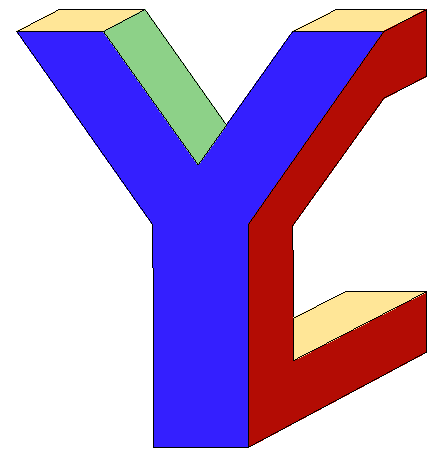
\includegraphics[height=1.5cm]{pictures/YC_logo.pdf} \hfill
    %& \begin{minipage}[t]{0.3\textwidth}\center \vspace{-1cm}  %Huawei-SPbSU Open Day 2021
    %  \end{minipage}
    %& \hfill 
\includegraphics[height=1.5cm]{pictures/SPbGU_Logo.png}
  %\end{tabularx}
  \end{table}
  \titlepage
\end{frame}
}

\begin{frame}[fragile]
  \frametitle{Agenda}  
  \begin{itemize}
    \item Algebraic Path Problems
    \item GraphBLAS
    \item Our team
  \end{itemize}
\end{frame}


\begin{frame}[fragile]
  \frametitle{GraphBLAS API\footnote{\url{https://graphblas.org/}}$^,$\footnote{\url{https://graphblas.org/GraphBLAS-Pointers/}}}
  \begin{itemize}
    \item Graph-matrix duality
    \item Operations over matrices and vectors
    \begin{itemize}
      \item Parametrized by semiring-like structures
      \item Sparse data
      \item Parallel
    \end{itemize}
    \item High-performance implementations
    \begin{itemize}
      \item SuiteSparse:GraphBLAS
      \item GraphBLAST
      \item Huawei
      \item \ldots
    \end{itemize}
  \end{itemize}
\end{frame}



\begin{frame}[fragile]
  \frametitle{BFS-like Skeleton}

  \newcommand\colR{\cellcolor{red!20}}
  \newcommand\colB{\cellcolor{blue!20}}
  \newcommand\colG{\cellcolor{green!20}}

  \begin{minipage}{0.2\textwidth}
  \begin{tikzpicture}[shorten >=1pt,auto]
    \node[state] (q_0)                      {$0$};
    \node[state] (q_1) [above right=of q_0] {$1$};
    \node[state,fill=red!20] (q_2) [right=of q_0]       {$2$};
    \node[state] (q_3) [right=of q_2]       {$3$};
    \path[->]
    (q_0) edge  node {a} (q_1)
    (q_1) edge  node {a} (q_2)
    (q_2) edge  node {a} (q_0)
    (q_2) edge[bend left, above]  node {b} (q_3)
    (q_3) edge[bend left, below]  node {b} (q_2);
    \end{tikzpicture}
  \end{minipage}~\pause
  \tikzmark{xPos}{}
  \begin{minipage}{0.75\textwidth}    
    \begin{equation*}
      \left(\begin{array}{cccc}        
        0  & 0  & \colR 1 & 0 \\        
      \end{array}\right)
      \times    
      \left(\begin{array}{cccc}        
        0 & 1 & 0 & 0 \\
        0 & 0 & 1 & 0 \\
        \rowcolor{red!20}
        1 & 0 & 0 & 1 \\
        0 & 0 & 1 & 0 \\        
      \end{array}\right)
      =      
        \left(\begin{array}{cccc}        
          \colB 1 & 0  & 0 & \colB 1 \\        
        \end{array}\right)
    \end{equation*}
    \mycallout<2-3>[opacity=1]{$(xPos) + (2.9,0.4)$}{Current front}{2.5}
    \mycallout<2-3>[opacity=1]{$(xPos) + (5.9,1.1)$}{Adjacency matrix}{3.5}
    \mycallout<2-3>[opacity=1]{$(xPos) + (9.2,0.4)$}{New front}{2.5}
    \mycalloutR<2-3>[opacity=1]{$(xPos) + (4.3,0.2)$}{Semiring}{1.5}
  \end{minipage}

  \pause

  \begin{minipage}{0.2\textwidth}
    \begin{tikzpicture}[shorten >=1pt,auto]
      \node[state, fill=blue!20] (q_0)                      {$0$};
      \node[state] (q_1) [above right=of q_0] {$1$};
      \node[state, fill=red!20] (q_2) [right=of q_0]       {$2$};
      \node[state, fill=blue!20] (q_3) [right=of q_2]       {$3$};
      \path[->]
      (q_0) edge  node {a} (q_1)
      (q_1) edge  node {a} (q_2)
      (q_2) edge  node {a} (q_0)
      (q_2) edge[bend left, above]  node {b} (q_3)
      (q_3) edge[bend left, below]  node {b} (q_2);
      \end{tikzpicture}
    \end{minipage}~
    \begin{minipage}{0.75\textwidth}
    \begin{equation*}
      \left(\begin{array}{cccc}        
        \colB 1 & 0  & 0 & \colB 1 \\        
      \end{array}\right)
      \times
      \left(\begin{array}{cccc}        
        \rowcolor{blue!20}
        0 & 1 & 0 & 0 \\
        0 & 0 & 1 & 0 \\        
        1 & 0 & 0 & 1 \\
        \rowcolor{blue!20}
        0 & 0 & 1 & 0 \\        
      \end{array}\right)
      =      
        \left(\begin{array}{cccc}        
          0 & \colG 1  & \colG 1 & 0 \\        
        \end{array}\right)
    \end{equation*}

  \end{minipage}

\end{frame}

%\begin{tikzpicture}
%  \draw[step=0.5cm,black,very thin] (0,0) grid (5,5);
%  \fill[blue!15] (0,1) rectangle (1,2);
%  \draw (3.5,1.5) node{$v_1^0$};
%\end{tikzpicture}

\begin{frame}[fragile]
  \frametitle{Research areas}  
  \begin{itemize}
    \item High-performance graph analysis
      
    \item Path problems with constraints
    
    \item Graph databases
    
    \end{itemize}
\end{frame}

\begin{frame}[fragile]
  \frametitle{Team}  
  \begin{itemize}
      \item Semyon Grigorev (Lead)
      \vspace{-0.4cm}
      \begin{AutoMultiColItemize}
        \item PhD (2016)
        \item Associate professor (2016, SPbSU)        
        \item \href{s.v.grigoriev@spbu.ru}{s.v.grigoriev@spbu.ru}
        \item High-performance graph analysis
        \item Graph databases
        \item dblp: \href{https://dblp.org/pid/181/9903.html}{https://dblp.org/pid/181/9903.html}
      \end{AutoMultiColItemize}
      
      \vspace{-0.2cm}
      \item Ekaterina Shemetova
      \vspace{-0.4cm}
      \begin{AutoMultiColItemize}
        \item PhD student 
        \item Path problems with constraints
        \item Fine-grained complexity
        \item Dynamic graph problems
      \end{AutoMultiColItemize}

      \vspace{-0.2cm}
      \item Rustam Azimov
      \vspace{-0.4cm}
      \begin{AutoMultiColItemize}
        \item PhD student 
        \item Linear algebra based graph analysis
        \item GraphBLAS API
        \item Algebraic path problem
      \end{AutoMultiColItemize}

    \end{itemize}
\end{frame}

\begin{frame}[fragile]
  \frametitle{Team: Master Students}  
  \begin{itemize}
      \vspace{-0.2cm}
      \item Alexandra Istomina
      \vspace{-0.4cm}
      \begin{AutoMultiColItemize}
        \item Master student
        \item Fine-grained complexity
        \item Path problems with constraints
        \item Algebraic path problem
      \end{AutoMultiColItemize}

      \vspace{-0.2cm}
      \item Egor Orachev
      \vspace{-0.4cm}
      \begin{AutoMultiColItemize}
        \item Master student
        \item Linear algebra based graph analysis
        \item GraphBLAS API
        \item GPGPU programming
      \end{AutoMultiColItemize}

      \vspace{-0.2cm}
      \item Vladimir Kutuev
      \vspace{-0.4cm}
      \begin{AutoMultiColItemize}
        \item Master student
        \item Linear algebra based graph analysis
        \item GraphBLAS API
        \item Parallel programming
      \end{AutoMultiColItemize}

      \vspace{-0.2cm}
      \item Julia Susanina
      \vspace{-0.4cm}
      \begin{AutoMultiColItemize}
        \item Master student 
        \item Linear algebra based graph analysis
        \item Probabilistic graph analysis
        \item GPGPU programming
      \end{AutoMultiColItemize}

    \end{itemize}
\end{frame}


\begin{frame}[fragile]
  \frametitle{High-Performance Graph Analysis}
  \begin{itemize}
    \item Linear algebra based algorithms for graph analysis
    \begin{itemize}
      \item Parallel algorithms on CPU and GPGPU
      \item Sparse linear algebra for graph analysis
      \item GraphBLAS API\footnote{\href{https://graphblas.org/}{https://graphblas.org/}}
    \end{itemize} 
    \pause
    \item Research directions
    \begin{itemize}
      \item GraphBLAS-based algorithms design, implementation and evaluation
      \item Portable multi-GPGPU implementation of GraphBALS-like API      
      \item GraphBLAS API analysis
    \end{itemize}
  \end{itemize}
\end{frame}

\begin{frame}[fragile]
  \frametitle{Path Problems With Constraints: Algebraic Path Problems}  
    \begin{itemize}
      \item Semiring-like structures to specify constraints on paths
      \begin{itemize}
        \item Reachability --- boolean semiring
        \item Shortest paths --- tropical semiring
        \item \ldots
      \end{itemize}
      \pause
      \item Linear algebra friendly algorithms 
      \begin{itemize}
        \item Transitive closure using matrix-matrix multiplication
        \item APSP using matrix-matrix multiplication
        \item BFS-like traversals using matrix-vector multiplication
        \item \ldots
      \end{itemize}
      \pause
      \item Compositionality
      \begin{itemize}
        \item Having two semirings one can create a new one
        \item Single solution for similar problems
        \begin{itemize}
          \item Generic solution
          \item Configurable solution
        \end{itemize}
      \end{itemize}
    \end{itemize}     
\end{frame}

\begin{frame}[fragile]
  \frametitle{Formal Language Constraint Path Querying}
    \begin{itemize}
      \item Particular case of algebraic path problem
      \begin{itemize}
        \item Multiplication is not associative
        \item Multiplication is not commutative
        \item \ldots
      \end{itemize}
      \pause
      \item Examples
      \begin {itemize}
        \item Regular path querying (RPQ)
        \item Context-free path querying (CFPQ)
      \end{itemize}
    \pause    
    \item Applications 
    \begin{itemize}
      \item Graph analysis
      \item Interprocedural static code analysis
      \item Graph database querying
    \end{itemize}
    \pause
    \item Research directions
    \begin{itemize}
      \item New algorithms development
      \item Complexity analysis
      \item New classes of languages investigation
      \item High performance algorithms implementation and evaluation 
    \end{itemize}
  \end{itemize}
\end{frame}

\begin{frame}[fragile]
  \frametitle{Our Results}
    \begin{itemize}
      \item Tools
      \begin{itemize}
        \item \href{https://github.com/JetBrains-Research/spla}{Spla: sparse linear algebra framework for multi-GPU computations based on OpenCL}
        \item \href{https://github.com/JetBrains-Research/spbla}{SPbLA: library of GPGPU-powered sparse boolean linear algebra operations}    
        \pause
        \item \href{https://github.com/JetBrains-Research/CFPQ_PyAlgo}{CFPQ\_PyAlgo: set of GraphBLAS-based FLPQ algorithms}
        \item \href{https://github.com/JetBrains-Research/ldbc_graphalytics}{LDBC Graphalytics extension for evaluation of formal language constrained path querying}            
        \pause
        \item \href{https://github.com/JetBrains-Research/GLL4Graph}{GLL4Graph: CFPQ for Neo4j}
        \item \href{https://github.com/YaccConstructor/RedisGraph}{CFPQ for RedisGraph}
      \end{itemize}
      \item Papers (> 10)
      \begin{itemize}
        \item SPbLA: The Library of GPGPU-Powered Sparse Boolean Linear Algebra Operations (GrAPL@IPDPS)
        \item Evaluation of the context-free path querying algorithm based on matrix multiplication (GRADES-NDA@SIGMOD)
        \item Multiple-Source Context-Free Path Querying in Terms of Linear Algebra (EDBT, Core A)
        \item Context-free path querying by matrix multiplication (GRADES-NDA@SIGMOD)
      \end{itemize} 
    \end{itemize}
\end{frame}


\begin{frame}[fragile]
  \frametitle{Possible Ways for Collaboration}
    \begin{itemize}
      \item Algebraic Path Problem framework applicability for network analysis
      \begin{itemize}        
        \item Which constraints can be specified in terms of semirings?
        \begin{itemize}
          \item Length minimality
          \item Nodes to visit
          \item \ldots
        \end{itemize}
        \item Is it flexible enough?
      \end{itemize}
      \item High-performance network analysis
      \begin{itemize}        
        \item GraphBLAS-based solution
        \item Algorithms development and analysis
        \item Algorithms implementation and evaluation
      \end{itemize} 
    \end{itemize}
\end{frame}


\begin{frame}[fragile]
  \frametitle{Possible Ways for Collaboration}
    \begin{itemize}
      \item Algebraic Path Problem framework applicability for network analysis
      \begin{itemize}        
        \item Unstructured path problems and the making of semirings (https://link.springer.com/chapter/10.1007/BFb0028261)
        \item Efficient Algorithms for Path Problems with Gernal Cost Citeria (https://www.semanticscholar.org/paper/Efficient-Algorithms-for-Path-Problems-with-Gernal-Lengauer-Theune/3fd320d97db0a581952d2919587b112f8df57c0b)
        \item Path Problems in Networks https://www.morganclaypool.com/doi/abs/10.2200/S00245ED1V01Y201001CNT003
        \item 

        \begin{itemize}
          \item Length minimality
          \item Nodes to visit
          \item \ldots
        \end{itemize}
        \item Is it flexible enough?
      \end{itemize}
      \item High-performance network analysis
      \begin{itemize}        
        \item GraphBLAS-based solution
        \item Algorithms development and analysis
        \item Algorithms implementation and evaluation
      \end{itemize} 
    \end{itemize}
\end{frame}



%How it (may) works



\end{document}
